\documentclass[12pt, oneside]{book}

\usepackage[T2A]{fontenc}			% кодировка
\usepackage[utf8]{inputenc}			% кодировка исходного текста
\usepackage[english,russian]{babel}	% локализация и переносы

\usepackage{amsmath}

\usepackage{amsthm, mathrsfs, mathtools, amssymb}

\usepackage{geometry}
\geometry{verbose,a4paper,tmargin=2cm,bmargin=2cm,lmargin=2.5cm,rmargin=1.5cm}

%\usepackage{showframe}

\usepackage[colorlinks=true, linkcolor=black, urlcolor=black]{hyperref}

\author{Кортенко~A.~М.}
\title{Конспект курса}
\date{\today}

\newtheorem{definition}{Определение}[section]
\newtheorem{theorem}{Теорема}[section]
\newtheorem{ex}{Пример}[section]
\newtheorem*{remark}{Замечание}

\newcommand{\toP}{\xrightarrow[]{P}} % сходимость по вероятности
\newcommand{\toPN}{\xrightarrow[]{\text{п.н.}}} % сходимость почти наверное
\newcommand{\toD}{\xrightarrow[]{\text{d}}} % сходимость по распределению (слабая)

\begin{document}
  \pagestyle{plain}

  \tableofcontents

  \chapter{Лекция 1 - 2023-09-06 - Основные распределения МС}
\section{Гамма-распределение}
\[
  \gamma_{\alpha, \lambda} (x) = \begin{cases}
    \dfrac{\alpha^\lambda}{\Gamma(\lambda)} x^{\lambda-1} e^{-\alpha x}, x>0 \\
    0, x \leqslant 0
  \end{cases}, \lambda > 0, \alpha > 0.
\]

\subsection{Гамма-функция \texorpdfstring{$\Gamma(\lambda)$}{Gamma(lambda)} }
\begin{definition}
  $$\Gamma(\lambda) = \int_0^{+\infty} x^{\lambda-1} e^{-x} \, dx, \lambda > 0.$$
\end{definition}

\begin{itemize}
  \item $\Gamma(1) = \int_0^{+\infty} e^{-x} \, dx = 1$.
  \item $\Gamma(\frac{1}{2}) = \int_0^{+\infty} x^{-1/2} e^{-x} \, dx = 2 \int_0^{+\infty} e^{-x} \, d\sqrt{x} = 2 \int_0^{+\infty} e^{-y^2} \, dy = \sqrt{\pi}$.
  \item $\Gamma(\lambda+1) = \int_0^{+\infty} x^\lambda e^{-x} \, dx = 
    \left. - x^\lambda e^{-x} \right|_0^{+\infty} 
    + \int_0^{+\infty} \lambda x^{\lambda-1} e^{-x} dx 
    = \lambda \Gamma(\lambda)$.

  В частности, $\Gamma(n+1) = n!$. 
\end{itemize}

\begin{remark}
  \[
    \lambda = 1 \Rightarrow \Gamma_{\alpha, 1} = \begin{cases}
      \alpha e^{-\alpha x}, x>0 \\
      0, x\leqslant 0
    \end{cases}
  \]
\end{remark}

\section{Бета распределение}

\begin{definition}
  $\beta_{m, n} = \begin{cases}
    \dfrac{x^{m-1}  (1-x)^{n-1}}{B(m, n)}, 0 < x < 1 \\
    0, x \notin (0, 1)
  \end{cases}, m, n > 0$
\end{definition}

\begin{definition}
  $B(m, n) = \int\limits_0^1 w^{m-1} (1-w)^{n-1} dw, m, n>0$.
\end{definition}

\begin{remark}
  Частные случаи:
  \begin{itemize}
    \item $\beta_{1, 1} = \begin{cases}
        \frac{1}{B(1, 1)} = 1, 0<x<1 \\
        0, x\notin (0, 1)
      \end{cases}$ - равномерное распределение на $(0, 1)$.

    \item $\beta_{\frac{1}{2}, \frac{1}{2}} (x) = \begin{cases}
        \dfrac{1}{\pi \sqrt{x(1-x)}}, 0<x<1 \\
        0, x \notin (0, 1)
      \end{cases}$ - закон арксинуса
  \end{itemize}
\end{remark}

\subsection{Свойства бета-функции}

\begin{itemize}
  \item $B(m, n) = \int\limits_0^\infty \dfrac{u^{m-1}}{(1+u)^{m+n}} \, du$
    \begin{proof}
      \begin{multline*}        
        \int\limits_0^1 w^{m-1} (1-w)^{n-1} \, dw = \left[
                \begin{aligned}
                  w &= \frac{u}{1+u} \\
                  1-w &= \frac{1}{1+u} \\
                  dw &= \frac{1}{(1+u)^2} du
                \end{aligned}
              \right] = \\
              = \int\limits_0^\infty \dfrac{u^{m-1}}{(1+u)^{m-1} (1+u)^{n-1} (1+u)^2} \, du = \int_0^\infty \dfrac{u^{m-1}}{(1+u)^{m+n}} \, du.
      \end{multline*}
    \end{proof}

  \item $B(m, n) = \dfrac{\Gamma(m) \Gamma(n)}{\Gamma(m+n)}$
    \begin{proof}
      \begin{multline*}
        \Gamma(\lambda) = \int\limits_0^{+\infty} x^{\lambda-1} e^{-x} \, dx =
        \left[ \begin{aligned} x &= (1+u)v \\ dx &= (1+u) dv \end{aligned} \right] =
        \int\limits_0^{+\infty} (1+u)^\lambda v^{\lambda-1} e^{-(1+u)v} \, dv \\
        \Leftrightarrow
        \dfrac{\Gamma(m+n)}{(1+u)^{m+n}} = \int\limits_0^{+\infty} v^{m+n-1} e^{-(1+u)v} \, dv \Leftrightarrow %\\
        % \Leftrightarrow
        \dfrac{\Gamma(m+n) u^{m-1}}{(1+u)^{m+n}} = \int\limits_0^{+\infty} v^{m+n-1} u^{m-1} e^{-(1+u)v} \, dv\\
        \text{интегрируя по u: }
        B(m, n) \Gamma(m+n) = \int\limits_0^{+\infty} \int\limits_0^{+\infty} v^{m+n-1} u^{m-1} e^{-(1+u) v} \, dv \, du = \\
        = \int\limits_0^{+\infty} \int\limits_0^{+\infty} v^{m+n-1} u^{m-1} e^{-v} e^{-uv} \, dv \, du =
        \int\limits_0^{+\infty} v^{n-1} e^{-v} \, dv \int\limits_0^{+\infty} (uv)^{m-1} e^{-uv} \, d(uv) = \\
        = \Gamma(n) \Gamma(m)
      \end{multline*}
    \end{proof}

  \item $B(m+1, n+1) = \dfrac{1}{(m+k+1) C_{m+k}^m}$ - следует из предыдущего.
\end{itemize}

\section{Хи-квадрат распределение с n степенями свободы}

\begin{definition}
  \[
    p_{\chi^2(n)} (x) = \begin{cases}
       \dfrac{x^{\frac{n}{2} - 1}}{2^\frac{n}{2} \Gamma(\frac{n}{2})} e^{-\frac{n}{2}}, x>0 \\
       0, x\leqslant 0
    \end{cases}
  \]
\end{definition}

\subsection{Свойства хи-квадрат распределения}

\begin{itemize}
  \item $p_{\chi^2(1)} (x) = \begin{cases}
      \frac{1}{\sqrt{2\pi y}} e^{-\frac{y}{2}}, y>0 \\
      0, y\leqslant 0
    \end{cases}$ - совпадает с распределение квадрата стандартной нормально распределенной случайной величины.
    
    \begin{proof}
    
    \end{proof}

  \item Пусть $\xi_i$ независимы и распределены по стандартному нормальному закону. Тогда случайная величина $\eta = \sum_{i=1}^n \xi_i^2$ распределена по закону хи-квадрат с n степенями свободы.
  
    \begin{proof}
      % TODO proof 
    \end{proof}

  \item $p_{\chi^2(n)} = \gamma_{\frac{1}{2}, \frac{n}{2}} (x)$.
\end{itemize}

\section{Распределение Фишера-Снедекора F(m,n)}

\begin{definition}
  \[
    p_{F(m, n)} (x) = \begin{cases}
      \dfrac{m^\frac{m}{2} n^\frac{n}{2} x^{\frac{m}{2}-1}}{(n+mx)^\frac{m+n}{2} B(\frac{m}{2}, \frac{n}{2}}, x>0 \\
      0, x\leqslant 0
    \end{cases}
  \]
\end{definition}

% TODO left part of lection

  \chapter*{Лекция 2 (2023-09-13). Виды сходимости случайных величин. Предельные теоремы
теории вероятностей. Закон больших чисел}

Пусть на $(\Omega, \mathscr A, \mathsf P)$ задана случайная величина $\xi$ и
последовательность случайных величин $\xi_1, \xi_2, \dots$. Поскольку случайная
величина есть \textsl{функция} от элементарных исходов, имеет смысл говорить о
разных видах сходимости. Рассмотрим их.

\section{Сходимость почти наверное}

\begin{definition}\label{def:pn}
	Говорят, что последовательность случайных величин $ \{\xi_n\} $ \emph{сходится почти
	наверное} к случайной величине $ \xi $ и пишут $\xi_n \toPN \xi$, если
	\[
		P\left(\lim_{n\to\infty} \xi_n = \xi \right) = 1.
	\]
\end{definition}

\begin{ex}
  Пусть $\Omega = [0, 1]$, $\mathscr A$ --- $\sigma$-алгебра измеримых
	подмножеств, $\mathsf P(A) = \operatorname{mes} A$.

	Определим
	\[
	  \xi_n(\omega) = \begin{cases} 1, &0\leqslant \omega < 1/n,\\
	  0, &\text{иначе}. 
    \end{cases}
	\]
  Тогда
	\[
		\forall \omega \neq 0\quad \xi_n(\omega) \to 0,
	\]
	то есть
	\[
		P\left(\lim_{n\to\infty} \xi_n=0\right) = 1.
	\]
\end{ex}

\begin{dfnbis}{def:pn}
	\label{def:pnbis}
	Говорят, что последовательность случайных величин $ \{\xi_n\} $ \emph{сходится почти
	наверное} к случайной величине $ \xi $ и пишут $\xi_n \toPN \xi$, если для
	сколь угодно малого $ \varepsilon > 0 $ выполняется
	\[
		\lim_{n\to\infty} \mathsf P\left\{ \omega\colon \sup\limits_{m\geqslant n}
		|\xi_n-\xi| > \varepsilon \right\} = 0.
	\]
\end{dfnbis}

\begin{utv}
	Определения {\rm\ref{def:pn}} и {\rm\ref{def:pnbis}} эквивалентны.
\begin{proof}
  Первое утверждение эквивалентно следующему:
  \[
  		\mathsf P \left( \xi_n \not\to \xi \right) = 0.
  \]
 
	По оперделению пердела 
	\[
		(\xi_n \to \xi) = \bigcap_{r=1}^\infty \bigcup_{n=1}^\infty\bigcap_{m\geqslant n}
		\left( |\xi_m - \xi| \leqslant 1/r \right),
	\]
а значит, 
\[
	(\xi_n \not\to \xi) = \bigcup_{r=1}^\infty \bigcap_{n=1}^\infty \bigcup_{m\geqslant n}
	\left( |\xi_m - \xi| > 1/r \right).
\]
В нашем случае будем иметь 
\[
	P\left(\bigcup_{r=1}^\infty \bigcap_{n=1}^\infty \bigcup_{m\geqslant n} (|\xi_m -
	\xi| \leqslant 1/r)\right),
\]
то есть для всех $ r \geqslant 1 $ получим
\[
	P\left(\bigcap_{n=1}^\infty \bigcup_{m\geqslant n} \left( |\xi_m - \xi| > 1/r
	\right)\right) = 0.
\]

Обозначим
\[
	B_n := \left\{\sup_{m\geqslant n} |\xi_m - \xi| > 1/r\right\} =
\left\{\bigcup_{m\geqslant n} (|\xi_m - \xi| > 1/r)\right\}.
\]
Тогда для всех $ k $ $ B_{k+1}
\subset B_k $ и $ \bigcap_{n=1}^\infty B_n = \varnothing $. По теореме о
непрерывности вероятности 
\[
	\lim_{n\to\infty} P(B_n) =  
	\lim_{n\to\infty} P \left(\sup_{m\geqslant n} |\xi_m - \xi| > 1/r \right) = 0.
\]

\end{proof}
\end{utv}



\section{Сходимость по вероятности}
\begin{definition}
	Говорят, что последовательность случайных величин $ \{\xi_n \}$ \emph{сходится
	по вероятности} и пишут $\xi_n \toP \xi$, если
	\[
		\forall \varepsilon > 0 \quad \lim_{n\to\infty}
		\mathsf P\left\{\omega \colon|\xi_n-\xi|>\varepsilon\right\} = 0.
	\]
\end{definition}

\begin{theorem}
  Если последовательность случайных величин почти наверное сходится к случайной
	величине $ \xi $, то эта же последовательность будет сходиться к ней по
	вероятности:
	\[
		\xi_n \toPN \xi \Rightarrow \xi_n \toP \xi.
	\]
\end{theorem}

\begin{proof}
  Очевидно. %TODO: (proof)
\end{proof}

%\begin{remark*}
%  Обратное, вообще говоря, не верно.
%\end{remark*}
\begin{ex} Обратное, вообще говоря, неверно. Действительно, пусть $ \Omega = [0,
	1]$, $ \mathscr A $ --- $ \sigma $-алгебра измеримых подмножеств, $ \mathsf
	P(A) = \operatorname{mes} A $. Для $ 2^k \leqslant n < 2^{k+1} $ определим
	последовательность 
	\[
		\xi_n(\omega) = \begin{cases}
			1, & \frac{n-2^k}{2^k} < \omega < \frac{n+1-2^k}{2^k},\\
			0, & \text{иначе}.
		\end{cases}
	\]
Для любого $ \varepsilon \in (0, 1) $ в этом случае имеем 
\[
	P(|\xi_n| > \varepsilon ) = \frac{1}{2^k} \to 0 \quad \text{при } n\to\infty,
\]
при этом $ \xi_n(\omega) \not\to 0 $ ($ \mathsf P $-п. н.).	
\end{ex}

\begin{theorem}
  Если последовательность $\{ \xi_n \}$ монотонно убывает (возрастает) и $\xi_n \toP \xi$, то
	\[
		\xi_n \toPN \xi.
	\]
\end{theorem}
\begin{proof}
Пусть $ \{\xi_n\} $ монотонно убывает и $ \xi_n \toP 0 $ (в случае возрастания
рассматривается последовательность $ \{\xi_n - \xi\} $). Тогда 
\[
	\left( \sup_{m\geqslant n}|\xi_m - \xi| > \varepsilon \right) = \left(
	\sup_{m\geqslant n} |\xi_m| > \varepsilon \right) = \left( \sup_{m\geqslant}
\xi_m > \varepsilon \right) = (\xi_n > \varepsilon). 
\]

\end{proof}

\begin{theorem}
  Если $\xi_n \toP \xi$, то из последовательности $\{ \xi_n \}$ можно выбрать
	подпоследовательность $\{ \xi_{n_k} \}$ такую, что
	\[
		\xi_{n_k} \toPN \xi.
	\]
\end{theorem}
\begin{proof}
  Без доказательства. %TODO: (proof)
\end{proof}

\section{Сходимость по распределению (слабая)}

\begin{definition}\label{def:d}
  Говорят, что последовательность \emph{сходится по распределению} и пишут $\xi_n \toD \xi$ или $F_{\xi_n} (x) \Rightarrow F_\xi (x)$, если для любой непрерывной ограниченной функции $g(x)$ выполняется:
  \[
		\lim_{n\to\infty}\int\limits_{-\infty}^{+\infty} g(x) \,
		dF_{\xi_n}(x) =
		\int\limits_{-\infty}^{+\infty} g(x) \, dF_\xi(x),
\]
или, что то же самое, 
\[
	\lim_{n\to\infty} \mathsf M g(\xi_n) = \mathsf M g(\xi).
\]
\end{definition}

\begin{dfnbis}{def:d}
	\label{def:dbis}
  $F_{\xi_n} (x) \Rightarrow F_\xi(x)$, если $F_{\xi_n}(x) \to F_\xi(x)$ в
	каждой точке непрерывности $F_\xi(x)$. Значит,
\[
	P(\xi_n < x) \xrightarrow[]{n\to\infty} P(\xi<x).
\]
\end{dfnbis}

\begin{theorem}
	Определения {\rm \ref{def:d}} и {\rm \ref{def:dbis}} эквивалентны.
\end{theorem}
\begin{proof} 
	Без доказательства. %TODO: (proof)
\end{proof}



\section{Сходимость в среднем порядка r}
\begin{definition}
	Будем говорить, что последовательность случайных величин \emph{сходится в
	среднем порядка $ r $} к случайной величине $ \xi $ и писать $ \xi_n \toR \xi
	$, если  
	\[
	\lim_{n\to\infty}\mathsf M |\xi_n - \xi|^r = 0.
	\]
	
\end{definition}

\begin{utv}
	Сходимость к $ \xi $ в среднем порядка $ r $ влечёт
	\[
		\xi_n\toR\xi \implies \xi_n \toP \xi
	\]
	сходимость к $ \xi $ по вероятности.
\end{utv}
\begin{proof}
	Применим неравенство Чебышёва и получим 
	\[
			P_\xi(|\xi_n - \xi| \geqslant x) = P (|\xi_n - \xi|^r \geqslant x^r )
			\leqslant \frac{\mathsf M |\xi_n - \xi|^r}{x^r}.
	\]
\end{proof}

\begin{ex}[факультативно]
	Пусть $ \{\xi_n\} $ --- последовательность независимых случайных величин,
	распределённых по закону
	\begin{table}[h!]
		\centering
	\begin{tabular}{|c|c|c|}
		\hline
		$ \xi_n , x_n $ &0 &1 \\\hline
		$ P_\xi(\xi_n = x_n) $ & $ 1 - 1/n $ & $ 1/n $\\\hline
	\end{tabular}.
\end{table}

Тогда  
\[
		P(|\xi_n| > \varepsilon) = P(\xi_n = 1) = \frac{1}{n} \to 0,
\]
а значит, 
\[
		\xi_n \toP 0.
\]
С другой стороны
\begin{multline*}
	P(\xi_n \to 0) = P(|\xi_m| < \varepsilon, \forall m \geqslant n) \leqslant \\
	\leqslant P(|\xi_m| < \varepsilon, \forall n \leqslant m < N) = \prod_{m=0}^N
	P(\xi_m = 0) = \\
	= \frac{n-1}{n}\frac{n}{n+1}\ldots
	\frac{N-1}{N} = \frac{n-1}{N} \to 0
\end{multline*}
при $ N \to \infty $.
\end{ex}


\section{Предельные теоремы}
\begin{theorem}[неравенства Чебышёва]
Для любого $ x > 0 $ имеют место неравенства 
\[
		P(|\xi|\geqslant x) \leqslant \frac{\mathsf M |\xi|}{x}, \qquad
		P(|\xi-\mathsf M\xi|\geqslant x) \leqslant \frac{\mathsf D\xi}{x^2}.
\]
\end{theorem}
\begin{proof}
	\begin{gather*}
		|\xi| = |\xi|\cdot I_{(|xi| \geqslant x)} + |\xi| \cdot I_{(|\xi|<x)}
		\geqslant |\xi| \cdot I_{(|\xi|\geqslant x)} \geqslant x \cdot I_{(|\xi|
		\geqslant x)},\\
		\mathsf M|\xi| \geqslant \mathsf M \left[ x\cdot I_{(|\xi|\geqslant x)}
		\right] = x \mathsf M \left[ I_{(|\xi| \geqslant x)} \right]  = x P(|\xi|
		\geqslant x).
\end{proof}

\begin{corollary*} 
\[
		P(|\xi-\mathsf M\xi|< x) \geqslant 1 - \frac{\mathsf D\xi}{x^2}.
\]
\end{corollary*}

\begin{theorem}[закон больших чисел Чебышёва]
	Пусть $ \{\xi_n\} $ --- независимые случайные величины и существует
	такая константа $ c > 0 $, что все $\mathsf D \xi_i \leqslant c$,
	$i=\overline{1,2,\ldots, n}$. Тогда при любом $ \varepsilon > 0 $  
	\[
		\lim_{N\to\infty} P_\xi \left( \left| \frac{\xi_1 + \xi_2 + \ldots +
		\xi_N}{N} - \frac{\mathsf M \xi_1 + \mathsf M\xi_2 + \ldots + \mathsf
	M\xi_N}{n} \right| < \varepsilon \right) = 1.
	\]
\end{theorem}
\begin{proof}
  Пусть  
  \[
  		\zeta_N = \frac{\xi_1 + \xi_2 + \ldots + \xi_N}{N}.
  \]
  Тогда
	\begin{align*}
		\mathsf M \zeta_N &= \frac{1}{N}\sum_{k=1}^N \mathsf M\xi_k,\\
		\mathsf D\zeta_N &= \frac{1}{N^2}\sum_{k=1}^N \mathsf D \xi_k \leqslant
		\frac{c}{N}.
\end{proof}
Следовательно, 
\[
		P(|\zeta_N - \mathsf M\zeta_N| < x) \geqslant 1 - \frac{c}{x^2N} \to 1
\]
при $ N \to \infty $. Здесь используется сходимость по вероятности 
\[
	\frac{1}{N}\sum_{k=1}^N \xi_k -\frac{1}{N} \sum_{k=1}^N \mathsf M\xi_k \toP 0.
\]



\begin{theorem}[центральная предельная теорема]
	Если случайные величины $ \{\xi_n\} $ независимы, одинаково распределены и
	имеют конечные $ \mathsf M\xi_i = a $, $ \mathsf D\xi_i = \sigma^2 > 0 $, то 
	\[
		\lim_{n\to\infty} P_\xi \left( \frac{\xi_1 + \xi_2 + \ldots + \xi_n -
		na}{\sigma \sqrt n} < x \right)  = \Phi(x),
	\]
	где используется сходимость по распределению.
\end{theorem}
\begin{theorem}[Ляпунов]
Пусть случайные величины $ \xi_1, \xi_2, \ldots $ --- независимы, имеют конечные
моменты $ \mathsf M \xi_k = a_k $, $ \mathsf D\xi_k = b^2_k $, $ \mathsf
M|\xi_k-a_k|^3 = c^3_k $. Обозначим $ A_n = \sum^n_{k=1} a_k $, $ B^2_n =
\sum^n_{k=1} b^2_k $, $ C^3_n = \sum^n_{k=1}c^3_k $, причём $ c_n/B_n \to 0 $.
Тогда 
\[
	\lim_{n\to\infty} P \left( \frac{\xi_1+\xi_2+\ldots+\xi_n-A_n}{B_n} < x
		\right) = \Phi(x),
\]
где используется сходимость по распределению 
\[
		\frac{\xi_1+\xi_2+\ldots+\xi_n-A_n}{B_n} \toD \mathscr N(0,1).
\]
\end{theorem}
\begin{theorem}[Хинчин] 
	Пусть $ \xi_1,\xi_2,\ldots $ --- одинаково распределеннные случайные величины
	с конечным математическим ожиданием $ a $.

	Тогда при любом $ \varepsilon > 0 $ имеем  
	\[
		\lim_{N\to\infty} P \left( \left| \frac{\xi_1+\xi_2+\ldots+\xi_N}{N} - a
		\right| < \varepsilon \right)  = 1,
	\]
	где используется сходимость по вероятности  
	\[
			\frac{\xi_1+\xi_2+\ldots+\xi_N}{N} \toP a.
	\]
\end{theorem}
\begin{theorem}[Марков]
	Пусть $ \xi_1,\xi_2,\ldots $ --- последовательность случайных величин,
	удовлетворяющая условию  
	\[
		\lim_{n\to\infty} \frac{1}{n^2} \mathsf D [\sum_{k=1}^n \xi_k] = 0.
	\]
	Тогда при сколь угодно малом $ \varepsilon > 0 $ имеем 
	\[
		\lim_{N\to\infty} P \left( \left| \frac{\xi_1 + \xi_2 + \ldots + \xi_N}{N} -
		\frac{\mathsf M \xi_1 + \mathsf M\xi_2 + \ldots + \mathsf M \xi_N}{N}\right|
	< \varepsilon \right) = 1,
	\]
где используется сходимость по вероятности  
\[
		\frac{\xi_1 + \xi_2 + \ldots + \xi_n}{N} - \frac{\mathsf M\xi_1 + \mathsf
		M\xi_2 + \ldots + \mathsf M\xi_N}{N} \toP 0.
\]	
\end{theorem}

\begin{theorem}[необходимое и достаточное условие]
	Пусть $\{\xi_n\}$ --- последовательность случайных величин с $ \mathsf M\xi_k
	= a_k$. Тогда закон больших чисел имеет место тогда и только тогда, когда  
	\[
			\lim_{N\to\infty} P \left( \left| \frac{\xi_1 + \xi_2 + \ldots + \xi_N}{N} -
		\frac{\mathsf M \xi_1 + \mathsf M\xi_2 + \ldots + \mathsf M \xi_N}{N}\right|
	< \varepsilon \right) = 1,
	\]
где используется сходимость по вероятности  
\[
		\frac{\xi_1 + \xi_2 + \ldots + \xi_N}{N} - \frac{\mathsf M \xi_1 + \mathsf
		M\xi_2 + \ldots + \mathsf \xi_N}{N} \toP 0.
\]
\end{theorem}	

\begin{theorem}[усиленный закон больших чисел Колмогорова]
	Пусть $ \{\xi_n\} $ --- независимые и одинаково распределённые
	случайные величины. Для того чтобы  
	\[
			\frac{\xi_1 + \xi_2 + \ldots + \xi_n}{n} \toPN a,
	\]
	необходимо и достаточно, чтобы существовало конечное
	\[
		\mathsf M\xi_k = a < \infty,
	\]
	где используется сходимость почти наверное: 
	\[
			\frac{\xi_1+\xi_2+\ldots+\xi_n}{n} \toPN a.
	\]
\end{theorem}	

\section{Резюме}
\begin{figure}[h!]
	\centering
	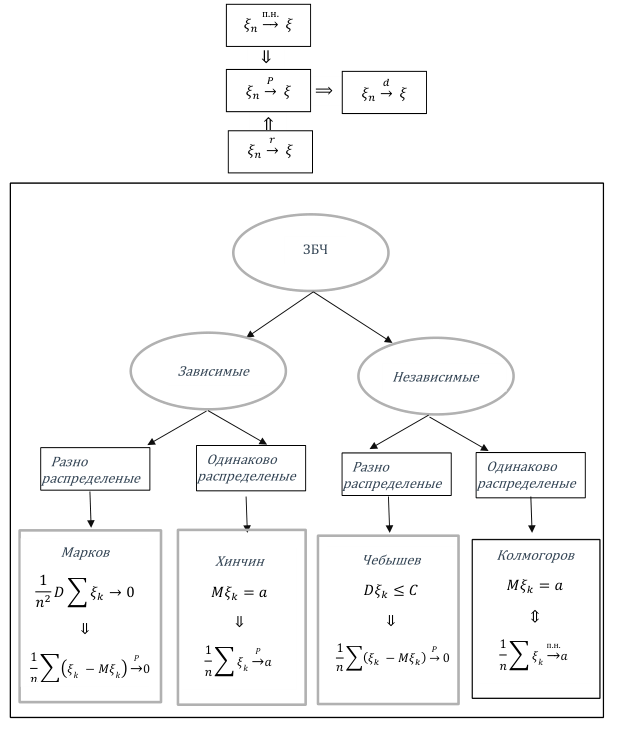
\includegraphics[width=0.8\textwidth]{Figures/resume.png}
	\label{fig:resume}
\end{figure}

  \chapter{Лекция 3 - 2023-09-20}
\section{Мотивация}
Пусть $ X = X_1, X_2, \ldots, X_n $ есть выборка (реализация случайной величины
$ \xi $, причём $ \{\xi_n\} $ независимы) из \textsl{известного}
распределения $ F(x, \theta) $, зависящего от \textsl{неизвестного} параметра $
\theta$.

\textsc{Задача}. Оценить значение параметра $ \theta $.

\begin{definition}
   Назовём функцию от выборки
	 \[
		 \widehat \Theta_n = f\left(x_1, x_2,\dots, x_n\right)
	 \]
	 \emph{оценкой параметра $\Theta$}, или \emph{статистикой}.
\end{definition}

Перечислим некоторые \textbf{свойства оценок}.
\begin{definition}
Оценку $ \widehat \Theta_n $ параметра назовём несмещённой, если 
\[
		\mathsf M \widehat \Theta_n = \theta.
\]
\end{definition}

%\begin{definition}
%  Оценка параметра $\widehat{D_n} = f(x_1, x_2, \dots, x_n)$.
%\end{definition}

\begin{definition}
  Оценка $\widehat{D_n}$ называется несмещенной, если $M[\widehat{D_n}]$.
\end{definition}

\[
  M f(\bar{x}) = \int\limits_{R_n} f(x_1, x_2, \dots, x_n) \prod\limits_{j=1}^{n} p_{x_i} (x_i) \, dx_1 dx_2 \dots dx_n.
\]

$$f(x_1, \dots, x_n) \toP 0, n \to \infty$$

Если $f(x_1, \dots, x_n) \toPN 0$, то $\hat{D_n}$ - силнльно состоятельная.

\begin{definition}
	Оценка $ \widehat \Theta_n $ называется \emph{асимптотически несмещённой},
	если  
	\[
		\mathsf M \widehat \Theta_n \to \theta \quad \text{при } n\to\infty.
	\]
\end{definition}

\begin{definition}
	Оценка $\widehat \Theta_n$ называется \emph{состоятельной}, если  
	\[
		\widehat \Theta_n \to \theta \quad \text{при } n\to\infty.
	\]
\end{definition}

\begin{definition}
Наконец, если  
\[
	\widehat \Theta_n \toPN \theta \quad \text{при } n\to\infty,
\]
то оценку $ \widehat \Theta_n $ называют \emph{сильно состоятельной}.
\end{definition}



%Пусть $x_1, \dots, x_n$ - выборка.
%$M X_i = a$.
%$$\hat{a_n} = ?$$

\section{Выборочное среднее}

\begin{definition}
	\emph{Выборочным средним} называют величину
	\[
		\hat a_n = \bar{X} = \frac{1}{n} \sum\limits_{i=1}^{n} x_i.
	\]
\end{definition}
Будем рассматривать $ \hat a_n $ как некоторую оценку математического ожидания
$ \mathsf M X_i = a $ рассматриваемой случайной величины. Обозначим кроме того
$ \mathsf D X_i = \sigma^2 $.

Перечислим \textbf{свойства выборочного среднего}.
\begin{enumerate}
	\item \textsc{Несмещённость}.
		\[
			M \bar{X} = M\left(\frac{1}{n} \sum\limits_{i=1}^{n} x_i\right) =
			\frac{na}{n} = a.
		\]
	\item \textsc{Сильная состоятельность}.
	\item \textsc{Дисперсия}. Дисперсия выборочного среднего стремится к нулю при увеличении $ n $.
		Действительно,  
		\[
			\mathsf D\bar X = \frac{1}{n^2} \sum_{i=1}^n \mathsf D X_i =
			\frac{\sigma^2}{n}.
		\]
		
\end{enumerate}

\section{Выборочная дисперсия (исправленная)}
\begin{definition} 
	\emph{Выборочной дисперсией} будем называть величину
\[ 
	S^2 = \frac{1}{n-1} \sum\limits_{i=1}^{n} \left( X_i-\bar{X}\right)^2.
\]
\end{definition}

Перечислим \textbf{свойства выборочной дисперсии}.
\begin{enumerate}
	\item Математическое ожидание выборочной дисперсии $ \mathsf M S^2 = \sigma^2
		$ равно истинной дисперсии. 
	\begin{multline*}
  \mathsf M S^2 = \frac{1}{n-1} \mathsf M\left[\sum_{i=1}^{n} \left(X_i - a - \left(\bar{X} - a\right)^2\right)^2 \right] = \\
  = \frac{1}{n-1} \sum \mathsf M (X_i-a)^2 - 2 \mathsf M\left[ \left(\bar{X} - a\right) \sum
	(X_i - a) \right] + \mathsf M (\bar{X} -a)^2 = \\
  = \frac{1}{n-1} \left[ n \sigma^2 - 2 n \mathsf M(\bar{X}-a)^2 + n \mathsf M (\bar{X}-a)^2 \right] = \\
  = \frac{1}{n-1} \left[ n \sigma^2 - n \frac{\sigma^2}{n} \right] = \sigma^2.
\end{multline*}
\item \textsc{Состоятельность}. 
\[
	S_n^2 = \frac{1}{n-1} \sum_{i=1}^n (X_i - \bar{X})^2 = \frac{n}{n-1} \left[
\frac{1}{n} \sum_{i=1}^n X_i^2 - \bar{X}^2 \right] \toPN \sigma^2 \quad
\text{при } n \to \infty.
\]
Действительно,
\[
	\frac{n}{n-1} \to 1, \qquad \bar X^2 \to a^2, 
\]
и, наконец,
\[
	\frac{1}{n} \sum_{i=1}^n X^2_i \toPN \sigma^2 + a^2
\]
в силу усиленного закона больших чисел.
\item \textsc{Дисперсия}.
\[
\mathsf D S^2 = \dfrac{\mu_4}{n} - \frac{\sigma^4 (n-3)}{n (n-1)} = O \left(\frac{1}{n}
\right),
\]
где $\mu_4 = \mathsf M X_i^4$ --- четвертый момент.
\end{enumerate}

\begin{theorem}[достаточное условие состоятельности]

Пусть $\widehat\Theta_n$ --- асимптотически несмешщенная оценка $\Theta$ и
$\mathsf D \bar\Theta_n \to 0$ при $ n \to \infty$.

Тогда $\widehat\Theta_n$ --- состоятельная оценка $\Theta$.
\end{theorem}
\begin{proof}
	Запишем условие состоятельности оценки $ \widehat\Theta_n $ в следующем виде:
\[
  | \widehat\Theta_n - \Theta| = |\widehat \Theta_n - \mathsf M \widehat\Theta_n
	+ \mathsf M \widehat\Theta_n
	- \Theta| \leqslant
	|\widehat\Theta_n - \mathsf M\widehat\Theta_n| + | \mathsf M\widehat\Theta_n -
	\Theta| \toP 0,
\]
где второе слагаемое стремится к нулю ввиду ассимптотической несмещённости $
\widehat\Theta_n $. Для сколь угодно малого $ \varepsilon > 0 $ имеем кроме того
\[
  P( | \widehat\Theta_n - \mathsf M \widehat\Theta_n| > \varepsilon) \leqslant
	\frac{|\widehat\Theta_n - \mathsf M
	\widehat\Theta_n| ^2} {\varepsilon^2} =  \frac{\mathsf D \widehat\Theta_n}
	{\varepsilon^2} \to 0 \quad \text{при } n \to\infty,
\]
что и доказывает утверждение.

\end{proof}



\section{Выборочная функция распределения}
\begin{definition}
	Назовём \emph{индикатором} функцию
\[
	I(x) = \begin{cases}1, &x>0,\\
	0, &x\leqslant 0.\end{cases}
\]
\end{definition}
Видно, что индикатор непрерывен слева.

\begin{definition}
	Назовём \emph{выборочной функцией распределения} функцию
	\[
		\widehat F_n (x) = \frac{1}{n} \sum_{i=1}^n I(x-X_i).
	\]
\end{definition}

\noindent Назовём некоторые из \textbf{свойств выборочной функции распределения}.
\begin{enumerate}
	\item \textsc{Несмещенность}.
\[
  \mathsf M \widehat F_n (x) = \mathsf M \frac{1}{n} \sum I(x-X_i)
\]

\item \textsc{Сильная состоятельность}.

\item \textsc{Теорема Гливенко -- Кантелли}.
	\begin{theorem}[Гливенко -- Кантелли] 

		\[
			\sup_x |\widehat F_n (x) - F(x)| \toPN 0.
		\]
	\end{theorem}
\begin{proof}
	б/д
	%TODO: (proof)

\end{proof}

\item \textsc{Неравенство Дворецкого -- Кифера -- Волфовица}.

\[
	P(\sup_x |\widehat F_n(x) - F(x)| > \varepsilon) \leqslant 2 e^{-2n
	\varepsilon^2}.
\]
\begin{proof}
	б/д
	%TODO: (proof)

\end{proof}
\begin{corollary*} 
	Возьмём для некоторого $ \alpha > 0 $
\[
		\varepsilon = \sqrt{ \frac{\ln 2/\alpha }{2n}}.
	\]
	Тогда
	\[
		P\left(\sup_x |\widehat F_n (x) - F(x)| \leqslant \varepsilon\right)
		\geqslant 1 - 2 e^{-2n \varepsilon^2} = 1-\alpha.
	\]
\end{corollary*}
Таким образом, с вероятностью $ 1 - \alpha $ имеем
\[
		\widehat F_n (x) - \varepsilon \leqslant F(x) \leqslant \widehat F_n(x) +
		\varepsilon,
\]
или более точно,
\begin{gather*}
	L(x) \leqslant F(x) \leqslant R(x), \quad \text{где}\\
		L(x) = \max \{ \widehat F_n(x) - \varepsilon,\, 0 \}, \qquad R(x) =
		\min \{ \widehat F_n(x) + \varepsilon, \,1 \}.
	\end{gather*}

\item \textsc{Общие свойства}:
	\begin{enumerate}
	\item Пределы  выборочной функции распределения при $ x \to \pm\infty $ равны
		соответственно
		\[
		\widehat F_n(+\infty) = 1, \qquad \widehat F_n(-\infty) = 0.
	\]
	\item Выборосная функция функция распределения $\widehat F_n(x)$ не убывает.
	\item Из первых двух свойств легко получаем 
	\[
			0 \leqslant \widehat F_n(x) \leqslant 1.
	\]
	
	\end{enumerate}
\end{enumerate}

\begin{theorem} Если выборка $x_1, \dots, x_n$ получена из закона распределения
	$F(x)$, то $\widehat F_n(x)$ есть дискретная случайная величина с распределением
\[
	P(\widehat F_n(x) = k/n) = C_n^k F(x)^k (1-F(x))^{n-k} 
\]
\end{theorem}
\begin{proof} 
	Из определения выборочной функции распределения
\[
	\widehat F_n \left(x\right) = \frac{1}{n} \sum_{i=1}^n I\left(x-X_i\right)
\]
сразу виден закон распределения Бернулли с вероятностью успеха $ p = F(x) $.

\end{proof}

\begin{corollary}
	\[
		\mathsf M \widehat F_n (x) = \frac{np}{n} = p = F(x).
	\]
\end{corollary}
\begin{corollary}
	\begin{multline*}
		\mathsf D \widehat F_n (x) = \frac{npq}{n^2} = \frac{F(x) (1 - F(x))}{n}
		\Leftrightarrow\\\Leftrightarrow
 \mathsf M (\widehat F_n(x) - F(x))^2 \to 0\Leftrightarrow\\
\Leftrightarrow \widehat F_n (x) \to F(x) \quad \text{(среднеквадратично при $
n\to\infty $)}.
\end{multline*}
\end{corollary}
\setcounter{corollary}{0}


\section{Порядковая статистика}
\begin{definition}
	Выборка, упорядоченная по возрастанию
	\[
		X_{(1)} \leqslant \dots \leqslant X_{(n)},
	\]
	 называется \emph{вариационным рядом}.
\end{definition}
\begin{definition}
	Член  вариационного ряда $ X_{(k)} $ называют \emph{$ k $-ой порядковой статистикой}.
\end{definition}

\begin{definition}
Назовём \emph{размахом выборки} число
\[
	\omega = X_{(n)} - X_{(1)}.
\]
\end{definition}

\begin{theorem}
	Если независимая выборка взята из генеральной совокупности с
функцией распределения $F(x)$, то функции распределения крайних членов
вариационного ряда и их совместная функция распределения имеют вид 
\begin{align*}
	\text{1. }F_{X_{(n)}}(x) &= [F(x)]^n,\\
	\text{2. }F_{X_{(1)}}(x) &= 1 - [1 - F(x)]^n,\\
	\text{3. }F_{X_{(1)}, X_{(n)}} (x, y) &= [F(y)]^n - [F(y)-F(x)]^n, \quad x < y.
\end{align*}
\end{theorem}
\begin{proof} Проведём доказательсто по всем пунктам.
	\begin{enumerate}
		\item Из независимости случайных величин и равенства $ X_{(n)} = \max\limits_i X_i $ вытекает соотношение
	\[
		F_{X_{(n)}}(x) = P \left( X_{(n)} < x \right) = P \left( \bigcap_{k=1}^n (X_k <
		x)\right) = \prod_{k=1}^n P(X_k < x) = [F(x)]^n.
	\]
\item Аналогично для $ X_{(1)} $ получим 
\[
	F_{X_{(1)}}(x) = 1 - P(X_{(1)} \geqslant x) = 1 - \prod_{k=1}^n P(X_k \geqslant
	x) = 1 - [1- F(x)]^n.
\]
\item В последнем случае 
\begin{multline*}
	F_{X_{(1)}, X_{(n)}}(x,y) = P(X_{(1)} < x, \, X_{(n)} < y) = \\ = P(X_{(n)} < y ) -
	P\left(X_{(1)} \geqslant x, \, X_{(n)} < y \right) = \\ =
	[F(y)]^n - P \left( \bigcap_{k=1}^n (x \leqslant X_k < y ) \right)  = \\ =
	[F(y)]^n - \prod_{k=1}^n P(x \leqslant X_k < y) = \\ =
	[F(y)]^n - [F(y) - F(x)]^n, \quad x < y.
\end{multline*}
\end{enumerate}
\end{proof}
\begin{corollary*}
	Если выборка взята из абсолютно непрерывного закона $F(x)$ с 
плотностью $p(x)$, то плотности распределения крайних членов вариационного ряда и их 
совместная плотность имеют вид 
\begin{align*}
	p_{X_{(n)}}(x) &= n[F(x)]^{n-1}p(x),\\
	p_{X_{(1)}}(x) &= n[1-F(x)]^{n-1}p(x),\\
	p_{X_{(1)}, X_{(n)}}(x, y) &= n(n-1)[F(y)-F(x)]^{n-2}p(x)p(y), \quad x < y.
\end{align*} %TODO: как получить последнее? (вписать формулу)
\end{corollary*}

\begin{theorem}
	Если независимая выборка взята из генеральной совокупности с
плотностью распределения $p(x)$, то плотность распределения $k$-ой порядковой
статистики имеет вид 
\[
	p_{X_{(k)}}(x) = n C^{k-1}_{n-1} \left[ F(x) \right]^{k-1} [1 - F(x)]^{n-k}
	p(x).
\]
\end{theorem}
\begin{proof}
	%TODO: поменять доказательство с инженерного на математическое (см. книгу
	%<<Порядковые статистики>>)
Зафиксируем $ x \in \mathbb R $ и выберем столь малое $ \Delta x $, что в
промежуток $ [x, x+ \Delta x) $ может попасть только один элемент выборки (закон
абсолютно непрерывный!). Тогда согласно полиномиальной схеме событие 
$(x \leqslant X_{(k)} < x + \Delta x)$ означает, что какие-то $ k - 1 $ элементов
выборки попали в промежуток $ (-\infty, x) $, 
один элемент в промежуток $[x, x + \Delta x)$, а остальные в $[x + \Delta x,
+\infty)$. Поскольку вероятности 
попаданий в эти множества равны $ F(x) $, $ p(x)\Delta x $ и $(1 - F(x + \Delta
x))$ соответственно, то  
\begin{multline*}
	F_{X_{(k)}}(x+\Delta x) - F_{X_{(k)}} (x) = P(x \leqslant X_{(k)} < x + \Delta
	x) = \\ =
	\frac{n!}{(k-1)!1!(n-k)!} [F(x)]^{k-1} p(x) \Delta x [1 - F(x + \Delta
	x)]^{n-k} = \\ =
	n C^{k-1}_{n-1} [F(x)]^{k-1} [1 - F(x + \Delta x)]^{n-k} p(x)\Delta x.
\end{multline*}
Завершим доказательство делением на $ \Delta x $ и переходом к пределу при $
\Delta x \to 0 $.

\end{proof}



\section{Примеры}
\begin{ex}
	Пусть дана выборка объёма $ n $ из показательного закона с параметром $ \alpha
	$. Тогда
	\[
		p_{X_{(1)}}(x) = n(1 - (1 - e^{-\alpha x}))^{n-1} \alpha e^{-\alpha
		x} = n \alpha e^{-n\alpha x}.
	\]
\end{ex}
\begin{ex}
	Найдём математическое ожидание и дисперсию $ X_{(k)} $, если выборка получена
	из равномерного распределения на $ [0, a] $. 

	Математическое ожидание минимального члена вариационного ряда равно
	\begin{multline*}
		\mathsf M X_{(1)} = \frac{n}{a }\int\limits_{0}^{a} x\cdot \left( 1 - \frac{x}{a}
		\right)^{n-1}\,dx \to \left[ \begin{aligned} u &= 1 - x/a \\ dx &= -a\,du
		\end{aligned}\right] \to an \int\limits_{0}^{1} \left( 1 - u \right) \cdot
		u^{n-1}\,du =\\=
		\frac{an}{n+1} \left. \left( 1 - \frac{x}{a} \right)^{n+1} \right|^a_0 - a
			\left.\left( 1 - \frac{x}{a} \right)^n \right|^a_0 = - \frac{an}{n+1} + a
				= \frac{a}{n+1}.
	\end{multline*}
	
	Математическое ожидание максимального члена вариационного ряда равно 
	\[
	\mathsf M X_{(n)} = \frac{n}{a}\int\limits_{0}^{a} x
	\left(\frac{x}{a}\right)^{n-1}\,dx = \frac{an}{n+1} \left.\left( \frac{x}{a}
	\right)^{n+1} \right|^a_0 = \frac{an}{n+1}.
	\]
	Отсюда видно, что $ X_{(n)} $ --- асимптотически несмещённая оценка параметра
	$ a $.

	Наконец, 
	\begin{multline*}
		\mathsf M X_{(k)} = \frac{n}{a}\int\limits_{0}^{a} x\cdot C^{k-1}_{n-1}
		\left(\frac{x}{a}\right)^{k-1} \left( 1 - \frac{x}{a} \right)^{n-k}\,dx = \\
		= an C^{k-1}_{n-1} \int\limits_{0}^{1}
		u^k(1-u)^{n-k}\,du = 
		an C^{k-1}_{n-1} B(k+1, n-k+1)  = \\ = a \frac{(n-1)!n}{(k-1)! (n-k)!}
		\frac{\Gamma(k+1) \Gamma(n-k+1)}{\Gamma(n+2)} = \frac{ak}{n+1},
	\end{multline*}
	где $ u = x/a $.
\end{ex}

  \chapter{Лекция 4 - 2023-09-27 - Методы получения точечных оценок: моментов, максимального
правдоподобия. Свойства точечных оценок.}

\section{Вероятности для вариационного ряда}

\begin{theorem}
  $X_1, X_2, \dots, X_n$ - независимыя выборка из з.р. $F(X)$

  тогда $F_{X_{(n)}} = (F(x))^n$, $F_{X_{(1)}} = 1 - (1-F(x))^n$.

  если имеется плотность $p(x)$, то $p_{X_{(n)}} = n (F(x))^{n-1} p(x)$, $p_{X_{(1)}} = n (1-F(x))^{n-1} p(x)$, $p_{X_{(1)}, X_{(n)}} = n (n-1) (F(y) - F(x))^{n-2} p(x) p(y)$.
\end{theorem}

\begin{proof}
  \begin{multline}
    F_{X_{(n)}} = P(X_{(n)} < x) = P\left(\bigcap_{k=1}^n (X_k < x)\right) = \prod_{k=1}^n P(X_k < x) = (F(x))^n\\
    F_{X_{(1)}} (x) = P(X_{(1)} < x) = 1 - P(X_{(1)} \geqslant x) = \dots = 1 - (1-F(x+0))^n = 1 - (1-F(x))^n \\
    F_{X_{(1)}, X_{(n)}} (x, y) = P(X_{(1)} < x, X_{(n)} < y) = P(X_{(n)} < y) - P(X_{(n)}, X_{(1)} \geqslant x) = \\
    F_{X_{(n)}} (y) - P(\bigcap_{k=1}^n (x \leqslant X_k < y)) = (F(y))^n - (F(y) - F(x))^n
    % \\
    % TODO: доказательство PX(1) X(n) (x, y)
  \end{multline}
\end{proof}

\begin{ex}
  $X_1, X_2, \dots, X_n ~ E(\alpha)$
  $F_{x_i} (x) = 1- e^{-\alpha x}, x\geqslant 0.$
  $F_{X_{(1)}} (x) = 1 - (1-1+e^{-\alpha x})^n = 1 - e^{-\alpha x} \Rightarrow X_{(1)} \sim E(n\alpha)$
\end{ex}

\begin{theorem}
  $X_1, X_2, \dots, X_n$ - независимая выборка из з.р. с плотностью $p(x)$.
  тогда $p_{X_{(k)}} = n C_{n-1}^{k-1} (F(x))^{k-1} (1-F(x))^{n-k} p(x)$.
\end{theorem}

\begin{proof}
  \[
    P(x\leqslant X_{(k)} < x+\Delta x) = \dfrac{n!}{(k-1)! (n-k)!} (F(x))^{k-1} p(x) \Delta x (1-F(x+\Delta x))^{n-k}
  \]
\end{proof}

\section{Методы построения точечных оценок параметров}

$X_1, X_2, \dots, X_n \sim F(x, \theta_1, \theta_2, \dots, \theta_n)$

\subsection{Метод моментов}

$\hat{\mu}_k = \frac{1}{n} \sum X_i^k$ - эмпирический момент k-го порядка.

$\mu_k = \int\limits_{-\infty}^{+\infty} x^k dF(x, \bar{\theta})$

По закону больших чисел: $\hat{\mu}_k \toPN \mu_k$

\[
\begin{cases}
  \hat{\mu}_1 = \mu_1(x, \bar{\theta}), \\
  \hat{\mu}_2 = \mu_2(x, \bar{\theta}), \\
  \dots = \dots \\
  \hat{\mu}_r = \mu_r(x, \bar{\theta})
\end{cases}
\]

\begin{ex}
  Пусть $X_1, \dots, X_n \sim E(\alpha)$.

  Тогда $\hat \mu_1 = \bar{X} = \frac{1}{\alpha} = \mu_1 \Rightarrow \alpha = \frac{1}{\bar{X}}$ - несмещённая.
  \begin{proof}
    $X_k \sim \alpha e^{-\alpha x} \equiv \gamma_{\alpha, 1}$
    Тогда $\xi = \sum X_k \sim \gamma_{\alpha, n}$.
    $M \hat \alpha_n = M \frac{n}{\xi} = \int\limits_0^{+\infty} \frac{n}{x} \dfrac{\alpha^n x^{n-1} e^{-\alpha x}}{\Gamma(n)} \, dx = \frac{n \alpha}{\Gamma(n)} \int\limits_0^{+\infty} (\alpha x)^{n-2} e^{-\alpha x} \, dx = \dfrac{n\alpha \Gamma(n-1}{\Gamma(n)} = \dfrac{n\alpha}{n-1} \to \alpha$
  \end{proof}
\end{ex}

\subsection{Оценки максимального правдоподобия}

$X_1, X_2, \dots, X_n \sim p(x, \bar\theta) \text{или} P(\xi = X_k)$

\begin{definition}
  $\mathcal{L} (X_1, X_2, \dots, X_n, \hat\theta) = $
  В случае непрерывной величины: $\mathcal{L} = \prod_{k=1}^n P(X_k, \hat \theta)$
  В случае дискретной: $\mathcal{L} = P(\xi_1 = X_1, \xi_2 = X_2, \dots, \xi_n = X_n) = \prod P(\xi_k = X_k)$

  $\mathcal{L}$ исследуется на максимум по параметру $\theta$.
\end{definition}

$\dfrac{\partial \mathcal{L}}{\partial \theta} = 0 \Leftrightarrow \frac{1}{\mathcal{L}} \dfrac{\ln \mathcal{L}}{\partial \theta} = 0$

\begin{ex}
  $X_1, X_2, \dots, X_n \sim Pois(\lambda)$
  $P(\xi=x_k) = \dfrac{\lambda^{X_k}}{(X_k)!} e^{-\lambda}$

  $\mathcal{L}(X_1, \dots, X_n, \lambda) = \prod \dfrac{\lambda^{X_k}}{(X_k)!} e^{-\lambda}$

  $\ln \mathcal{L} = \sum X_k \ln\lambda - n \lambda - \ln \prod (X_k)!$

  $\dfrac{\partial \ln \mathcal{L}}{\partial \lambda} = \dfrac{\sum X-k}{\lambda} - n = 0 \Rightarrow \bar{\lambda_n} = \frac{1}{n} \sum X_k$
\end{ex}

\begin{ex}
  $X_1, X_2, \dots, X_n \sim E(\alpha)$

  $\mathcal{L}(X_1, \dots, X_n, \alpha) = \prod \alpha e^{-\alpha x_k} = \alpha^n e^{-\alpha \sum x_k}$

  $\ln \mathcal{L} = n \ln\alpha - \alpha \sum x_k$

  $\dfrac{\partial \ln\mathcal{L}}{\partial \alpha} = \frac{n}{\alpha} - \sum x_k$
\end{ex}

\subsection{Сравнение оценок}

\begin{definition}
  Если $\hat \theta_n$ и $\widehat{\widehat{\theta}}_n$ - две несмещенные оценки параметра $\theta$.
  Если $D \hat\theta_n < D \hat\hat\theta_n$, то говорят, что $\hat\theta_n$ - более эффективна, чем $\hat\hat\theta_n$
\end{definition}

\begin{ex}
  $X_1, X_2, \dots, X_n \sim R[\theta-\frac{1}{2}, \theta+\frac{1}{2}]$

  $\hat\theta_n = \frac{1}{2} (X_{(1)} + X_{(n)})$
  
  $\Hat{\Hat{\theta}}_n = \bar X$

  $D\hat\theta_n = \dots = \dfrac{1}{8 (n+1) (n+2)} \sim \dfrac{c}{n^2}$

  $D\Hat{\Hat{\theta}}_n = \dfrac{1}{12n}$
\end{ex}

\begin{theorem}[Неравенство Рао-Крамера]
  Если $X_1, X_2, \dots, X_n$ - выборка из закона распределения с плотностью $p(x, \theta)$ и $\int\limits_R p(x, \theta) \, dx = 1$ допускает дифференцирование по $\theta$.
  Тогда $\forall$ несмещенной оценки $\hat\theta_n$ имеет место:
  $$D\hat\theta_n \geqslant \frac{1}{I_n(\theta)} = \frac{1}{n I_1(\theta)},$$
  где $I_n(\theta) = M\left( \dfrac{\partial \ln \mathcal{L}}{\partial \theta} \right)^2$ - информация Фишера,
    $I_1(\theta) = M\left( \dfrac{\partial\ln p(x, \theta)}{\partial\theta} \right)^2$
\end{theorem}

\begin{proof}
  $1 = \int\limits_{R^n} p(x, \theta) \, dx \Rightarrow 0 = \int\limits_{R^n} \dfrac{\partial p(x, \theta)}{\partial\theta} \, dx = \int\limits_{R^n} \dfrac{\ln p(x, \theta)}{\partial\theta} p(x, \theta) \, dx$

  $\hat\theta_n = \phi(X_1, X_2, \dots, X_n), \theta = \int_{R^n} \phi(x) p(x, \theta) \, dx \Rightarrow 1 = \int_{R^n} \phi(x) \dfrac{\partial \ln p(x, \theta)}{\partial\theta} p(x, \theta) \, dx$

  $\Rightarrow 1 = \int_{R^n} (\phi(x)-\theta) \dfrac{\partial \ln p(x, \theta)}{\partial \theta} p(x, \theta) \, dx$

  $1 \leqslant \int_{R^n} (\phi(x) - \theta)^2 p(x, \theta) \, dx \cdot \int_{R^n} (\dfrac{\partial\ln p(x, \theta)}{\partial\theta})^2 p(x, \theta) \, dx$

  $I_n(\theta) = M \left(\dfrac{\partial\ln L(X_1, X_2, \dots, X_n, \theta)}{\partial\theta}\right)^2 = D \dfrac{\partial \ln L}{\partial\theta} = \sum D\dfrac{\partial \ln p(x_k, \theta)}{\partial\theta} = n I_1(\theta)$

  $\ln L(X, \theta) = \sum \ln p(x_k, \theta)$
\end{proof}

\begin{ex}
  $X_1, \dots, X_n \sim R[\theta-1/2, \theta+1/2]$

  $p(x, \theta) = I(\theta-1/2 \leqslant x \leqslant \theta+1/2)$

  $1 = \int\limits_{-\infty}^{+\infty} I \, dx$ - не допускает дифференцирование по параметру.
\end{ex}

\begin{ex}
  $X_1, X_2, \dots, X_n \sim E(\alpha)$

  $p(x, \alpha) = \alpha e^{-\alpha x}$

  $I_1(\alpha) = M (\dfrac{\partial\ln p(X_1, \alpha)}{\partial\alpha})^2$

  $\ln p(X_1, \alpha) = \ln \alpha - \alpha X_1$

  $\dfrac{\partial \ln p}{\partial\alpha} = \frac{1}{\alpha} - X_1$

  $I_1(\alpha) = M (\frac{1}{\alpha} - X_1)^2 = D X_1 = \dfrac{1}{\alpha^2}$
\end{ex}

Вывод: $\forall$ несмещенной оценки $\hat\alpha_n$: $D \hat\alpha_n \geqslant \dfrac{1}{n \frac{1}{\alpha^2}} = \frac{\alpha^2}{n}$ 


  \chapter{Лекция 5 - 2023-10-04 - Достаточные статистики. Критерий факторизации}
\section{Достаточные статистики}
Пусть $ X_1, X_2, \ldots, X_n $ --- выборка из распределения, зависящего от
параметра $ \bar \theta $ (реализация случайного вектора $ \bar \xi = (\xi_1,
\xi_2, \ldots, \xi_n) $ с независимыми компонентами).

\begin{definition}
  Вектор-функция $\bar t = \bar t(X_1, X_2, \dots, X_n)$ называется \emph{достаточной
	статистикой} для оценки параметра $\bar{\theta}$, если условная функция
	распределения
	\[
		F_{\bar \xi} (X_1, X_2, \dots, X_n\, | \,\bar{t} (\xi_1, \dots, \xi_n)
		= \bar t)
	\]
	не зависит от $\bar\theta$ при любых значениях $\bar t$. 
\end{definition}

\begin{remark*}
Статистика $ \bar t $ является достаточной для оценки параметра $ \theta $, если
\begin{enumerate}
	\item \textsc{Дискретный случай}. Условные вероятности 
	\[
			P(\xi_1 = X_1, \xi_2 = X_2, \ldots, \xi_n = X_n\, \mid \, \bar t(\bar \xi) = \bar
			t)
	\]
	не зависят от $ \theta $ при любых значениях $ \bar t $.
\item \textsc{Непрерывный случай}. Условные плотности  
\[
	p_{\bar \xi} (X_1, X_2, \ldots, X_n\, |\,\bar t(\bar \xi) = \bar t)
\]
не зависят от $ \theta $ при любых значениях $ \bar t $.
\end{enumerate}

\end{remark*}

\begin{ex}
  Пусть $X_1, X_2, \dots, X_n$ распределены по Бернулли с вероятностью успеха $p$
	(последовательность 0 и 1).

	Докажем, что статистика $\sum_{k=1}^n X_k$ достаточна для оценки параметра $p$.
Найдём условные вероятности
  \begin{multline*}
		P\left(\xi_1 = X_1, \dots, \xi_n = X_n\,\Big|\, \sum_{k=1}^n \xi_k =
		t\right) = \\
		= \frac{P(\xi_1 = X_1, \dots \xi_n = X_n, \sum \xi_k = t)}{P\left(\sum_{k=1}^n \xi_k = t\right)} = \\
    = \begin{cases}
			p = 0, &t \neq \sum_{k=1}^n X_k, \\
			\frac{ p^t (1-p)^{n-t} }{ C_n^t p^t (1-p)^{n-t} } = \frac{1}{C_n^t}, &t
			= \sum_{k=1}^n X_k.
    \end{cases}
  \end{multline*}
	Действительно, знаменатель по теореме Бернулли равен $ C^t_n p^t(1-p)^{n-1} $.
	Числитель равен нулю, если $ t \ne \sum_{k=1}^n $ и $ p^t(1-p)^{n-t} $ в ином
	случае.

	Таким образом, условная вероятность в любом случае не зависит от $ p $.
\end{ex}

\begin{theorem}[критерий факторизации]
  Если $X_1, X_2, \dots, X_n \sim F(x, \bar\theta)$, то $\bar t = \bar t (X_1,
	\dots, X_n)$ является достаточной статистикой для оценки $\bar\theta$ тогда и
	только тогда, когда 
  \[
    \mathscr{L}(X_1, X_2, \dots, X_n, \bar\theta) = h(X_1, \dots, X_n)
		g(\bar\theta, \bar t (X_1, X_2, \dots, X_n)),
  \]
  где $h$ не зависит от $\theta$, $g$ не зависит от $X_1, X_2, \dots, X_n$
	(разве что через $\bar t$)
\end{theorem}

\begin{proof}
	Проведём доказательство в обе стороны.
	\begin{enumerate}
		\item $\boxed{\Leftarrow}$ Пусть
			\[
				\mathscr L(X_1, X_2, \ldots, X_n, \theta) = g\left(\bar \theta, \bar t(X_1,
				X_2, \ldots, X_n) \right)h(X_1, \ldots, X_n).
			\]

			Имеем
  \begin{multline*}
    P(\xi_1 = X_1, \dots, \xi_n = X_n \, | \, \bar t (\xi_1, \dots, \xi_n) = \bar t)
    = \\ = \frac{P(\xi_1=X_1, \dots, \xi_n = X_n, \bar t(X_1, \dots, X_n) = \bar
		t_0)}{P(\bar t(\xi_1, \dots, \xi_n) = \bar t_0)}.
  \end{multline*}
При $ \bar t(X_1, X_2, \ldots, X_n) \neq \bar t_0$ полученное выражение,
очевидно, равно нулю. Рассмотрим случай $ \bar t(X_1, X_2, \ldots, X_n) = \bar
t_0 $. Тогда числитель будет равен функции правдоподобия $ \mathscr L(X_1,
\ldots , X_n, \bar \theta) $, а знаменатель 
\[
		P(\bar t(\xi_1, \ldots, \xi_n) = \bar t) = \sum_{\bar Z \colon \bar t(\bar
		Z) = \bar t_0} P(\xi_1 = Z_1, \ldots, \xi_n = Z_n) = \sum_{\bar Z\colon \bar
		t(\bar Z) = \bar t_0}\mathscr L(Z_1, \ldots, Z_n, \bar \theta). 
\]

Следовательно, для рассматриваемого случая имеем
\begin{multline*}
    P(\xi_1 = X_1, \dots, \xi_n = X_n \, | \, \bar t (\xi_1, \dots, \xi_n) =\\=
		\frac{P(\xi_1 = X_1, \ldots, \xi_n = X_n)}{\sum P(\xi_1 = Z_1, \ldots, \xi_n = Z_n)} =\\= \frac{h(X_1, \dots, X_n)
		g(\bar \theta, \bar t(X_1, \dots, X_n))}{\sum h(Z_1, \dots, Z_n)
		g(\bar\theta, \bar t(Z_1, \dots, Z_n)} = \frac{h(X_1, \dots, X_n)}{\sum h(Z_1,
		\dots, Z_n)},
\end{multline*}
где суммирование, как и прежде, производится по таким $ \bar Z $, что $ \bar
t(\bar Z) = \bar t_0 $. Результат не зависит от $ \bar \theta $, что и
требовалось доказать.
\item $\boxed{\Rightarrow}$
  Докажем, обратно, что если вероятность
	\[
		P(\xi_1 = X_1, \dots, \xi_n = X_n \,| \,\bar
		t(\xi_1, \dots, \xi_n)
		= \bar t)
	\]
	не зависит от $\bar \theta$, то $\mathscr{L}$ факторизуется. Действительно, в
	случае $ \bar t_0 = \bar t(X_1, \ldots, X_n) $
  \begin{multline*}
    \mathscr{L} (X_1, \dots, X_n, \bar\theta) = P_{\bar\theta} (\xi_1 = X_1,
		\dots, \xi_n = X_n) =\\= P_{\bar\theta} (\xi_1 = X_1, \dots, \xi_n = X_n \,
		|\, \bar
		t(\bar\xi) = \bar t) \cdot P(\bar t(\bar\xi) = \bar t).
  \end{multline*}
  Первый множитель не зависит от $\bar\theta$, второй зависит от $X_1, \dots,
	X_n$ только через $\bar t(X_1, \dots, X_n)$.

\end{proof}

\begin{remark}
  \begin{align*}
		\mathscr{L} &= h(X_1, \dots, X_n) g(\bar\theta, \bar t(X_1, \dots, X_n),\\
		\ln \mathscr{L} &= \ln h + \ln g,\\
		\frac{\partial \ln g}{\partial \bar \theta} &= \frac{\partial \ln \mathscr{L} (\bar\theta, \bar t(X_1, \dots,
	X_n))}{\partial \bar\theta}.
  \end{align*}
  $\Rightarrow$ ОМП функция от $\bar t(X_1, \dots, X_n)$
  % что значит последняя строка?
  % TODO не понял о чём это замечание, скорее всего ошибка
\end{remark}

\begin{ex}
	Пусть $X_1, \dots X_n \sim \operatorname{Pois}(\lambda)$, 
  \[
    P(X_1, \dots, X_n, \lambda) = P_\lambda (\xi_1=X_1, \dots, \xi_n=X_n) =
		\prod_{k=1}^n P(\xi_k = X_k) = \prod_{k=1}^n \frac{\lambda^{X_k}}{(X_k)!}
		e^{-\lambda} =
		\frac{\lambda^{\sum X_k}}{\prod_{k=1}^n (X_k)!}  e^{-n\lambda},
  \]
	а значит, $\sum_{k=1}^n X_k$ --- достаточная статистика для оценки $\lambda$
	(как и $\bar X$).
\end{ex}

\begin{ex}
  Пусть $X_1, \dots, X_n \sim N(a, \sigma)$.
  \begin{multline*}
		\mathscr{L} (X_1, \dots, X_n, a, \sigma) = \prod_{k=1}^n \frac{1}{\sqrt{2\pi}
		\sigma} \exp\left(-\frac{(X_k-a)^2}{2\sigma^2}\right) =\\= 
		\left(\frac{1}{\sqrt{2\pi}\sigma} \right)^n
		\exp\left(-\frac{1}{2\sigma^2} \sum_{k=1}^n (X_k-a)^2\right) = \\ =
		\left(\frac{1}{\sqrt{2\pi}\sigma}\right)^n \exp\left(-\frac{1}{2\sigma^2}
			\left(\sum_{k=1}^n
		X_k^2 - 2a \sum_{k=1}^n X_k + na^2\right)\right).
  \end{multline*}
  Здесь достаточной статистикой для $ (a, \sigma) $ будет $(\sum X_k^2, \sum
	X_k)$.

  В то же время
	\[
		\sum_{k=1}^n (X_k-a)^2 = \sum_{k=1}^n (X_k - \bar X + \bar X - a)^2 =
		\sum_{k=1}^n (X_k-\bar X)^2 + (\bar X - a)^2 n,
	\]
	поэтому пара
	\[
		\left(\bar X,\, S^2 = \frac{1}{n-1} \sum_{k=1}^n (X_k-\bar X)^2\right)
	\]
	является достаточной статистикой для $\sigma$ при известном $a$.
\end{ex}

\begin{ex}
	Пусть $X_1, \dots, X_n \sim \operatorname{Par}(\alpha, \theta)$. Плотность
	равна
	\[
		p(x, \theta, \alpha) = \frac{\alpha}{\theta}
		\left(\frac{\theta}{x}\right)^{\alpha+1}, \quad x\geqslant 0.
	\]

	Найдём функцию правдоподобия и вычленим достаточную статистику:
  \[
		\mathscr{L} (X_1, \dots, X_n, \alpha, \theta) = \prod_{k=1}^n \frac{\alpha}{\theta}
		\left(\frac{\theta}{x}\right)^{\alpha+1} I(X_k \geqslant 0) = \frac{\alpha^n
		\theta^{\alpha n}}{(\prod X_k)^{\alpha+1}} I(X_{(1)}\geqslant 0) \cdot 1.
  \]
Следовательно, 
  $(X_{(1)}, \prod X_k)$ --- достаточная статистика для закона Паретто.
\end{ex}

\section{Интервальные оценки (доверительные интервалы)}
Пусть $X_1, \dots, X_n$ --- выборка из распределения с плотностью $p(x,
\theta)$, а $1-\alpha$ --- \emph{уровень доверия}.

\begin{definition}
	\emph{Доверительным интервалом} для одномерного параметра $\theta$ с 
доверительной вероятностью $1  - \alpha$ называется любой интервал $(\theta_1, \theta_2)$, 
содержащий истинное значение параметра с вероятностью $1 - \alpha$.  
\end{definition}


\subsection{Принцип построения доверительных интервалов}
\begin{enumerate}
  \item Находим статистику $\eta = \varphi(X_1, \dots, X_n, \theta)$, закон
		распределения  которой $F_\eta (x)$ известен точно или приближенно и не
		зависит от $\theta$.
  \item Находим квантили $t_{\alpha/2}$ и $t_{1-\alpha/2}$, при этом
    \[ 
			F_\eta(t_{\alpha/2})  = \alpha/2,\quad F_\eta(t_{1-\alpha/2}) = 1 -
			\alpha/2.
		\]
		Тогда
    \[
      P(t_{\alpha/2} < \varphi(X_1, \dots, X_n, \theta) < t_{1-{\alpha/2}}) =
			F_\eta (t_{1 - \alpha/2}) - F_\eta (t_{\alpha/2}) = 1- \alpha
    \]
  \item Неравенство  
  \[
		t_{\alpha/2} < \varphi(X_1, \ldots, X_n, \theta) < t_{1-\alpha/2}
  \]
		разрешается относительно $\theta$: 
		\[
			\ubar \varphi(X_1, \ldots, X_n, \alpha) < \theta < \bar\varphi(X_1,
			\ldots, X_n, \alpha).
		\]
		Обозначив $ \theta_1 = \ubar\varphi(X_1, \ldots, X_n, \alpha) $, $ \theta_2
		= \bar\varphi(X_1, \ldots, X_n, \alpha)$, получаем доверительный интервал
		уровня $ 1 - \alpha $.
\end{enumerate}

\begin{ex}[для неизвестного $ a $ при известном $ \sigma $]
  Пусть $X_1, \dots, X_n \sim N(a, \sigma_0)$, где $\sigma_0$ известна.

  Тогда по методу моментов $\hat a = \bar X$. Отсюда
  \[
		\bar X = \frac{1}{n} \sum_{k=1}^n X_k \sim N\left(a,
		\frac{\sigma_0}{\sqrt{n}}\right).
  \]

	Следовательно, распределение
	\[
		\frac{\bar X - a}{\sigma_0} \sqrt{n} \sim N(0, 1)
	\]
не зависит от параметра $a$.

Получили
  \[
		-u_{1-\alpha/2} = u_{\alpha/2} &< \frac{\bar X - a}{\sigma_0} \sqrt{n} <
		u_{1-\alpha/2}, 
	\]
	или
	\[
		\bar X - \frac{u_{1-\alpha/2}}{\sqrt{n}} &< a < \bar X +
		\frac{u_{1-\alpha/2}}{\sqrt{n}}.
	\]
 \end{ex}

 \begin{ex}[для неизвестного $ \sigma $ при известном $ a $]
  Рассмотрим противоположный случай. Пусть $X_1, \dots, X_n \sim N(a_0,
	\sigma)$,
	и параметр $a_0$ известен.

	В этом случае
	\[
		\mathscr{L} (X_1, \dots, X_n, \sigma) = \prod_{k=1}^n \frac{1}{\sqrt{2\pi}
		\sigma} \exp\left(-\frac{(X_k - a)^2}{2\sigma^2}\right) =
		\left(\frac{1}{\sqrt{2\pi}\sigma}\right)^n \exp\left(-\frac{1}{2\sigma^2}
		\sum_{k=1}^n (X_k-a)^2\right).
	\]
	Следовательно, $\sum_{k=1}^n (X_k-a)^2$ (вместе с $ S_0^2 = 1/n \sum_{k=1}^n(X_k - a_0)^2 $) будет достаточной статистикой.

	При этом, как легко заметить,
	\[
		\sum\limits_{k=1}^n \frac{(X_k-a)^2}{\sigma^2} = \frac{S^2_0 n}{\sigma^2}
		\sim \chi^2 (n).
	\]

	Найдём квантили и разрешим неравенство:
  \begin{gather*} 
		\chi^2_{\alpha/2} (n) < \sum_{k=1}^n \frac{(X_k - a_0)^2}{\sigma^2} <
		\chi^2_{1 - \alpha/2} (n), \\
		\frac{\sum_{k=1}^n (X_k-a_0)^2}{\chi^2_{1 - \alpha/2} (n)} < \sigma^2 <
		\frac{\sum_{k=1}^n (X_k - a_0)^2}{\chi^2_{\alpha/2}(n)}.
  \end{gather*}
\end{ex}

\begin{ex}
  Произведено $n=36$ измерений, $\bar X = 9.3 \text{кОм},  \sigma_0 = 2
	\text{кОм}$. Найти доверительный интервал $1- \alpha = 0.95$ для оценки
	параметра $a$.

\[
  0.95 = P\left(\bar X - \frac{u_{0.975} \cdot 2}{\sqrt{36}} < a < \bar X + \frac{u_{0.975} \cdot 2}{\sqrt{36}}\right) \Leftrightarrow a \in (8.65, 9.95)
\]
\end{ex}

\begin{ex}[на показательный закон]
	Пусть
  $X_1, \dots, X_n \sim E(\lambda)$.
  Достаточной статистикой  будет $\hat \lambda = \frac{1}{\bar X}$. Докажем
	сначала, что
  \[
		2\lambda \sum_{k=1}^n X_k \sim \chi^2(2n).
	\]

	Действительно, имеем
	\[
		X_k \sim \lambda e^{-\lambda x} \Rightarrow \eta = 2\lambda X_k \sim \frac{1}{2}
		e^{-\frac{x}{2}} \equiv \chi^2 (2).
	\]

	Найдём квантили и разрешим неравенство: 
	\begin{gather*}
		\chi^2_{\alpha/2}(2n) < 2\lambda\sum_{k=1}^n X_k <
		\chi^2_{1-\alpha/2}(2n),\\
	\frac{\chi^2_{\alpha/2}(2n)}{2 n\bar X } < \lambda <
	\frac{\chi^2_{1-\alpha/2}(2n)}{2 n \bar X}.
	\end{gather*}
\end{ex}

\subsection{Приближенные доверительные интервалы}
  Пусть $X_1, \dots, X_n \sim F(x, \theta), \M_\theta X_i = a(\theta), \D_\theta
	X_i = d(\theta)$, и $n$ велико. 

	Тогда согласно центральной предельной теореме статистика
\[
	\frac{\sum_{i=1}^n X_i - n a(\theta)}{\sqrt{n d(\theta)}} \approx N(0, 1)
\]
в пределе распределена по стандартному нормальному закону, что даёт приближённое
равенство
\[
	P\left(u_{1 - \alpha/2} < \frac{\sum_{i=1}^n X_i - n a(\theta)}{\sqrt{n d(\theta)}}<
	u_{1-\alpha/2}\right) \approx 1 - \alpha.
\]

\begin{ex}[на биномиальный закон, $ k $ известно]
  Пусть $X_1, \dots, X_n \sim B(k, p)$, но $k$ известно, а $ p $ неизвестно.

	Известно, что 
	\[
		\M X_k = kp, \quad \D X_k = k p (1-p).
	\]
В этом случае
\[
	\frac{\sum_{k=1}^n X_k - n k p}{\sqrt{nkp(1-p)}} \in (-u_{1-\alpha/2}, u_{1-\alpha/2})
\]
с вероятностью, стремящейся к $ 1 - \alpha $. Чтобы не решать квадратные
неравенства, заменим ещё $ p $ под корнем в
знаменателе оценкой $\hat p = \frac{\bar X}{k}$ (потеря точности невелика). 

Найдём квантили и разрешим неравенство:
\begin{gather*}
	-u_{1-\alpha/2}\cdot \sqrt{nk \frac{\bar X}{k} \left(1 - \frac{\bar X}{k}\right)} <
	\sum_{k=1}^n X_k -
	nkp < u_{1-\alpha/2} \cdot \sqrt{nk \frac{\bar X}{k} \left(1 - \frac{\bar X}{k}\right)}, \\
	\frac{\bar X}{k} - \frac{u_{1-\alpha/2}\cdot \sqrt{\frac{\bar X}{k} \left(1 - \frac{\bar
	X}{k}\right)}}{\sqrt{nk}} < p < \frac{\bar X}{k} + \frac{u_{1-\alpha/2}
\cdot \sqrt{\frac{\bar X}{k} \left(1 - \frac{\bar X}{k}\right)}}{\sqrt{nk}}.
\end{gather*}
\end{ex}

  \chapter{Лекция 6 - 2023-10-11}

\section{Доверительные интервалы для параметров нормального закона}

$X_1, \dots, X_n \sim N(a, \sigma)$

\begin{theorem}
  Если $X_1, \dots, X_n \sim N(a, \sigma)$, то статистика $\bar X$ и $\dfrac{(n-1) S^2}{\sigma^2} = \dfrac{1}{\sigma^2} \sum\limits_{k=1}^n (X_k-\bar X)^2$ независимы и $\bar X \sim N(a, \dfrac{\sigma}{\sqrt{n}}$, $\dfrac{(n-1) S^2}{\sigma^2} \sim \chi^2(n-1)$
\end{theorem}

\begin{theorem}[Лемма]
  $n = 1, \eta = a \xi, p_\eta(y) = \dfrac{1}{|a|} p_\xi(y/a)$.
  Если $p_{\bar \xi} (\bar x)$ - плотность СВ $\bar\xi$, СВ $\bar\eta = A\xi$, $\exists A^{-1}$
  $p_{\bar\eta} (\bar y) = |det A|^{-1} p_{\bar\xi} (A^{-1} \bar y)$
\end{theorem}
\begin{proof}
  $$p(\bar\xi \in B) = p(A\xi \in AB) = p(\eta \in AB)$$
  $$ p(\xi \in B) = \int_B p_\xi (\bar x) \, d\bar x
  = \left|\, \begin{aligned}
    \bar x &= A^{-1} \bar y \\
    \bar y &= A \bar x \\
    d\bar x &= |det(A^{-1})| d\bar y
  \end{aligned} \,\right| 
  = \int_{AB} p_\xi(A^{-1} \bar y) |det A_{-1}| d\bar y 
  \Rightarrow p_{\bar \eta} (\bar y)
  = p_{\bar\xi} (A^{-1} \bar y) |det A^{-1}|$$
\end{proof}


\begin{proof}[доказательство первой теоремы]
  $X_1, \dots, X_n \rightarrow X_1', \dots, X_n'$
  $$\bar X' = \dfrac{1}{n} \sum\limits_{k=1}^n X_k' = \dfrac{1}{n} \sum \dfrac{(X_k - a)}{\sigma} = \dfrac{\bar X - a}{\sigma}$$
  $$\vec{X}' = (X_1', \dots, X_n')^T$$
  $$p_{\bar X'} (x) = \dfrac{1}{(\sqrt{2\pi})^n} e^{-\dfrac{1}{2} \bar x^T \bar x}$$
  $$\bar Y = C \bar X', C - \text{ортог}$$
  $$Y_1 = \dfrac{1}{\sqrt{n}} \sum X_k' = \sqrt{n} \bar X' = \dfrac{\bar X - a}{\sigma} \sqrt{n}$$
  $$Y_1^2 = n (\bar X')^2$$
  $$p_{\bar Y} (y) = |det C|^{-1} p_{\bar X} (C^{-1} \bar y) = \dfrac{1}{(\sqrt{2\pi})^n} e^{-\dfrac{1}{2} (C^{-1} \bar y)^T C^{-1} \bar y} = \dfrac{1}{(\sqrt{2\pi})^2} e^{-\dfrac{1}{2} \bar y^T \bar y}$$
  
  \begin{multline*}
    ? \bar X и \dfrac{(n-1) S^2}{\sigma^2}; \\
    \dfrac{(n-1) S^2}{\sigma^2} \dfrac{1}{\sigma^2} \sum (X_k-\bar X)^2 = \dfrac{1}{\sigma^2} \sum ((X_k - a) - (\bar X - a))^2 =\\
    \sum \dfrac{(X_k-a)^2}{\sigma^2}-2 \dfrac{\bar X - a}{\sigma^2} \sum (X_k-a) + \dfrac{n}{\sigma^2} (\bar X - a)^2 = \\
    \sum \dfrac{(X_k-a)^2}{\sigma^2} - n \left(\dfrac{\bar X-a}{\sigma}\right)^2  = \sum (X_k')^2 - n (\bar X')^2 = \sum Y_k^2 - Y_1^2 = \\ 
    \sum\limits_{k=2}^n Y_k^2 \sim \chi^2(n-1)
  \end{multline*}
  $$\bar X = \sigma (\bar X' + a) = \sigma \left(\sqrt{\dfrac{Y_1}{n}} + a\right)$$
\end{proof}

\section{Доверительные интервалы}

Для $\sigma$ при неизвестном a:
\begin{align*}
  \dfrac{(n-1) S^2}{ \sigma^2 } &\sim \chi^2(n-1) \\
  \chi^2_{\alpha/2} (n-1) < \dfrac{(n-1) S^2}{\sigma^2}& < \chi^2_{1 - \alpha/2} (n-1) \\
  \sqrt{\dfrac{(n-1) S^2}{\chi^2_{1 - \alpha/2}(n-1)}} < \sigma& < \sqrt{\dfrac{(n-1) S^2}{\chi^2_{\alpha/2} (n-1)}}
\end{align*}

2. Дов. инт для а при неизвестном $\sigma$
\begin{align*}
  \sqrt{n} \dfrac{\bar X - a}{S} &= \sqrt{n} \dfrac{\dfrac{\bar X - a}{\sigma}}{\dfrac{S}{\sigma}} = \sqrt{n} \dfrac{\dfrac{\bar X - a}{\sigma}}{\sqrt{\dfrac{1}{n-1} \dfrac{(n-1) S^2}{\sigma^2}}} \sim t(n-1) \\
  S &= \sqrt{S^2} \\
  -t_{1 - \alpha/2} (n-1) &= t_{\alpha/2} (n-1) < \sqrt{n} \dfrac{\bar X - a}{\sigma}& < t_{1-\alpha/2} (n-1) \\
  \bar X - \dfrac{t_{1-\alpha/2}(n-1) S}{\sqrt{n}} < a& < \bar X + \dfrac{t_{1-\alpha/2}(n-1) S}{\sqrt{n}}
\end{align*}

3. Доверительный интервал для разности мат ожиданий при известной дисперсии
$X_1, \dots, X_n \sim N(a, \sigma_x)$, $Y_1, \dots, Y_m \sim N(b, \sigma_y)$, $\sigma_x, \sigma_y$ - независимы.
? $a-b$

\begin{multline*}
  \dfrac{\bar X - \bar Y - (a-b)}{\sqrt{\dfrac{\sigma_x^2}{n} + \dfrac{\sigma_y^2}{n}}} \sim N(0, 1) \\
  M(\bar X - \bar Y - (a-b)) = (a-b) - (a-b) = 0 \\
  D(\dfrac{\bar X - \bar Y - (a-b)}{\sqrt{\dfrac{\sigma_x^2}{n} + \dfrac{\sigma_y^2}{n}}} = \dfrac{D \bar X + D \bar Y}{\sigma_x^2 / n + \sigma_y^2 / m} = \dfrac{\sigma_x^2 / n + \sigma_y^2 / m}{\sigma_x^2 / n + \sigma_y^2 / m} = 1 \\
  - u_{1-\alpha/2} < \dfrac{\bar X - \bar Y - (a-b)}{\sqrt{\sigma_x^2 / n + \sigma_y^2 / m}} < u_{1-\alpha/2} \\
  \bar X - \bar Y - u_{1-\alpha/2} \sqrt{\sigma_x^2 / n + \sigma_y^2 / m}< a-b < \bar X - \bar Y + u_{1-\alpha/2} \sqrt{\sigma_x^2 / n + \sigma_y^2 / m} 
\end{multline*}

4. Для разности матожиланий при неизв диспресия
$X_1, \dots, X_n \sim N(a, \sigma)$, $Y_1, \dots, Y_m \sim N(b, \sigma)$, $\sigma$ - неизвестн.
\begin{multline*}
  \dfrac{\bar X - \bar Y - (a-b)}{\sigma \sqrt{1/n + 1/m}} \sim N(0, 1) \text{и не зависит от $\dfrac{(n-1)S_x^2}{\sigma^2} + \dfrac{(m_1) S_y^2}{\sigma^2}$} \\
  \dfrac{\bar X - \bar Y - (a-b)}{\sqrt{1/n + 1/m} \sqrt{\dfrac{1}{n+m-2} \dfrac{(n-1) S_x^2 + (m-1)S_y^2}{\sigma^2}}} \sim t(n+m-2)\\
\dfrac{\bar X - \bar Y - (a-b)}{\sqrt{1/n + 1/m}} \sim N(0, 1) \\
\dfrac{(n-1) S_x^2 + (m-1)S_y^2}{\sigma^2} \sim \chi^2(n+m-2) \\
(a-b) \in (\bar X - \bar Y - \delta, \bar X - \bar Y + \delta), где \\
\delta = t_{1-\alpha/2} (n+m-2) \sqrt{\dfrac{n+m}{nm(n+m-2)}} \sqrt{(n-1)S_x^2 + (m-1) S_y^2}
\end{multline*}

5. доверительный интервал для отношения дисперсий
$X_1, \dots, X_n \sim N(a, \sigma_x)$, $Y_1, \dots, Y_m \sim N(b, \sigma_y)$

\begin{multline*}
  \dfrac{\sigma_y^2}{\sigma_x^2} \dfrac{S_x^2}{S_y^2} = \dfrac{(n-1) S_x^2 / \sigma_x^2}{(m-1) S_y^2 / \sigma_y^2} \dfrac{m-1}{n-1} \sim F(n-1, m-1) \\
(m-1) S_y^2 / \sigma_y^2 \sim \chi^2(m-1), (n-1) S_x^2 / \sigma_x^2 \sim \chi^2(n-1) \\
f_{\alpha/2} (n-1, m-1) < \dfrac{\sigma_y^2 s_x^2}{\sigma_x^2 s_y^2} < f_{1-\alpha/2} (n-1, m-1) \\
\dfrac{S_x^2}{S_y^2 f_{1-\alpha/2} (n-1, m-1)} < \dfrac{\sigma_x^2}{\sigma_y^2} < \dfrac{s_x^2}{s_y^2 f_{\alpha/2} (n-1, m-1)}
\end{multline*}

6. Дов интервал для отношения дисперсий при изв a, b

\begin{multline*}
  \dfrac{S_{x0}^2}{\sigma_x^2} = \dfrac{1}{n}\sum \dfrac{(X_k-a)^2}{\sigma_x^2}\sim \chi^2(n) \\
  \dfrac{S_{y0}}{\sigma_y^2} = \dfrac{1}{m} \sum \dfrac{(Y_k - b)^2}{\sigma_y^2} \sim \chi^2 (m)
\end{multline*}

% TODO дописать 6 

  \section{Лекция 7 - 2023-10-18}

\[
P(A|D) = \dfrac{P(D|A) P(A)}{P(D)}
\]

\begin{ex}
  Пусть имеется монета с вероятностью выпадения решки x ($x \sim R[0, 1]$).
  $D_{hk} = $ монета подброшена n раз и в k опытах выпала решка.
  
  H_k задают дискретный закон:
  $$P(\xi = x_j | D) = \dfrac{P(D|\xi=x_j) P(\xi=x_j)}{P(D)}$$

  $H_\theta$ - набор 

  $$P(H_\theta | D) = \dfrac{P(D|H_\theta) P(H_\theta)}{P(D)}$$

  Терминология:
  \begin{itemize}
    \item $P(H_\theta |D)$ - апостериорная вероятность ($\dots$)
    \item $P(D|H_\theta)$ - likelihood правдоподобия
  \end{itemize}
\end{ex}

\begin{ex}
  \begin{tabular}{|c|c|c|}
    & успех & неудача \\
    $H_1$ & 1/3 & 2/3 \\
    $H_2$ & 1/2 & 1/2
  \end{tabular}

   % TODO: дописать этот пример
   % в лекциях Облаковой описано всё текстом, а на лекции было много формул

\end{ex}

Если $H_\theta$ - набор абсолютно-непрерывных законов.

\[
  p(x|D) = \dfrac{P(D|x) p(x)}{P(D)} \propto P(D|x) p(x)
\]

$p(x)$ - априорная плотность

$P(D|x)$ - функция правдоподобия

\begin{ex}
  x - вер успеха, $x \sim R[0, 1]$

  $D_{nk}$

  \begin{multline*}
    p(x|D_{nk}) \propto P(D_{nk} | x) p(x) \\
    P(D_{nk} | x) = x^k (1-k)^{n-k} \\
    \sum X_j = k \\
    p(x|D_{nk}) = \dfrac{x^k (1-k)^{n-k}}{B(k+1, n-k+1)} - \text{бета распределение}
  \end{multline*}

  \begin{align*}
    D_{11} &\Rightarrow p(x|D_{11}) = \dfrac{x}{B(2, 1)} = 2x \\
    D_{22} &\Rightarrow p(x|D_{22}) = \dfrac{x^2}{B(3, 1)} = 3x^2 \\
    D_{21} &\Rightarrow p(x|D_{21}) = \dfrac{x (1-x)}{B(2, 2)} = 6x(1-x)
  \end{align*}
\end{ex}

\begin{theorem}[Колмогорова-Блэкуэлла]
  Пусть $X_1, \dots, X_n \sim p(x, \theta)$ и $\bar t = \bar t(X_1, \dots, X_n)$ - достаточная статистика для оценки $\theta$.
  Если $\tilde \theta_n$ - любая несмещенная оценка $\theta$. $\hat \theta_n = M(\tilde \theta_n | \bar t(X_1, \dots, X_n))$ - также несмещенная оценка и $D\hat \theta _n \leqslant D \tilde \theta_n$.
\end{theorem}

Свойства условного МО (как СВ)
$M(\xi|\eta) = M(\xi | \eta = y) |_{y=\eta}$ (то есть рассматриваем как будто y зафиксировано, а потом подставляем вместо y какую-то СВ)
\begin{enumerate}
  \item $MM(\xi | \eta) = M\xi$ 
  \item $M(\xi \cdot g(\eta) | \eta) = g(\eta) \cdot M(\xi)$
  \item в частности $M\left(g(\eta) | \eta\right) = g(\eta)$
  \item $M(\xi - M(\xi | \eta))^2 = \min_g M(\xi - g(\eta))^2$
\end{enumerate}

\begin{proof}
  \begin{multline*}
    M\hat\theta_n = MM(\tilde \theta_n | \bar t(X_1, \dots, X_n)) = M(\tilde \theta_n) = \theta \\
    M\tilde \theta_n 
    = M(\tilde \theta_n - \theta)^2
    = M(\tilde\theta_n - \hat\theta_n + \hat\theta_n - \theta)^2
    = M(\tilde\theta_n - \hat\theta_n)^2 + M(\hat\theta_n-\theta)^2 + 2 M(\tilde\theta_n - \hat\theta_n)(\hat\theta_n - \theta) =\\
    = M(\tilde\theta_n - \hat\theta_n)^2 + D\tilde\theta_n \leqslant 0 \\
  \end{multline*}

  Доказательство того, что последнее слагаемое действительно 0:
  \begin{multline*}
    M((\tilde\theta_n - \hat\theta_n)(\hat\theta_n-\theta) | \bar t(X_1, \dots, X_n))
    = |\text{$(\hat\theta_n - \theta)$ - функция от $\bar t$}| = \\
    = (\hat\theta_n - \theta) \left[ M(\tilde\theta_n|\bar t) - M(\har\theta_n | \bar t) \right]
    = \dots
    = 0
  \end{multline*}
  % TODO возможно нужно получше расписать
\end{proof}

\begin{ex}
  Пусть $X_1, \dots, X_n \sim N(a, 1)$
  $\tilde a_n = X_1$, $M\tilde a_n = MX_1 = a$, $D\tilde a_n = D X_1 = 1$

  $\hat a_n = \bar X$, $M \hat a_n = M\bar X = a$, $D \hat a_n = 1/n$

  Достаточная статистика:
  \begin{multline*}
    \mathcal{L}(X_1, \dots, X_n, a)
    = \dfrac{1}{(\sqrt{2\pi})^n} e^{-\dfrac{1}{2} \sum (X_k - a)^2}
    = \dfrac{1}{(\sqrt{2\pi})^n} e^{-\dfrac{1}{2} (\sum X_k^2 + a \sum X_k - na^2 / 2)} \\
    \bar t = \sum X_k
  \end{multline*}

  \begin{multline*}
    M(X_1 | \sum X_k) = M(X_2 | \sum X_k) = \dots = M(X_n | \sum X_k) \\
    \sum X_k = M(\sum X_k | \sum X_k) = n M(X_1 | \sum X_k) \Rightarrow \\
    \Rightarrow M(X_k) = \dfrac{1}{n} \sum X_k
  \end{multline*}

  \begin{multline*}
    p_{X_1} (x | \bar x = y) = \dfrac{p_{X_1, \bar X} (x, y)}{p_{\bar X} (y)} \\
    (X_1, \bar X) - \text{нормальный вектор} \\
    MX_1 = a, DX_1 = 1, M\bar X = a, D\bar X = \dfrac{1}{n} \\
    \operatorname{cov} (X_1, \bar X) = \dfrac{1}{n} \sum_{k=1}^n \operatorname{cov} (X_1, X_k) = \dfrac{1}{n} (1 + 0 + \dots + 0) = \dfrac{1}{n} \\
    \Sigma = \begin{pmatrix}
      1 & 1/n \\
      1/n & 1/n
    \end{pmatrix},
    |\Sigma| = (n-1) / n^2,
    \Sigma^{-1} = \dfrac{1}{|\Sigma|} \begin{pmatrix}
      1/n & - 1/n \\
      -1/n & 1
    \end{pmatrix} \\
    p_{X_1, \bar X} (x, y)
    = \dfrac{1}{2\pi \sqrt{(n-1) / n^2}} e^{- \dfrac{n^2}{2(n-1)} \left( \dfrac{1}{n}(x-a)^2 - \dfrac{2}{n} (x-a)(y-a) + (y-a)^2 \right) } \\
    p_{X_1} (x | \bar X = y) = \dfrac{N}{N} \sim N() 
    % TODO дописать последнюю строчку
  \end{multline*}
\end{ex}

\subsection{Эффективные оценки}

Неравенство Рао-Крамера: $D\hat \theta_n \geqslant 1 / (n I_1(\theta))$

\begin{def}
  $e(\hat \theta_n) = \dfrac{1}{n I_1(\theta) D(\hat\theta_n)} \leqslant 1$ - эффективность.
  Оценка называется эффективной, если $e(\hat\theta_n) = 1$
\end{def}

\begin{ex}
  Пусть $X_1, \dots, X_n \sim N(a, \sigma_0)$, $\sigma_0$ - известно.
  
  $\hat a_n = \bar X$, $D\hat\theta_n = \dfrac{\sigma_0^2}{n}$

  \begin{multline*}
    \mathcal{L} (X_1, \dots, X_n, a)
    = \dfrac{1}{(\sqrt{2\pi})^n \sigma_0^n} e^{-\dfrac{1}{2\sigma_0} \sum (X_k-a)^2 } \\
    \ln \mathcal{L} = -\dfrac{n}{2} \ln 2n - n \ln \sigma_0 - \dfrac{1}{2\sigma_0^2} \\
    \dfrac{\partial \ln \mathcal{L}}{\partial a} = - \dfrac{1}{\sigma_0^2}\sum (X_k-a) \\
    \dfrac{\partial \ln \mathcal{L}_1}{\partial a} = - \dfrac{1}{\sigma_0^2} \\
    I_1(a) = M( \dfrac{\partial \ln \mathcal{L}_1}{\partial a}  )^2
    = M \dfrac{1}{\sigma_0^4} (X_1-a)^2
    = \dfrac{1}{\sigma_0^4} \sigma_0^2 = \dfrac{1}{\sigma_0^2} \\
    e(\bar X) = \dfrac{1}{n I_1 D\bar X} = \dots = 1
  \end{multline*}
  $\Rightarrow$ $\bar X$ - эффективная оценка.
\end{ex}

\begin{theorem}[о связи эффективных оценок и достаточных статистик]
  Если $\hat\theta_n = \bar t(X_1, \dots, X_n)$ - несмещенная и эффективная оценка $\theta$, построенная по выборке $X_1, \dots, X_n \sim p(x, \theta)$. $p(x, \theta)$ - удовлетворяет условиям регулярности, то $\bar t(X_1, \dots, X_n)$ - достаточная статистика.
\end{theorem}
\begin{proof}
  $1 = \int_{R^n} p(\bar X, \theta) \, d\bar X$ - можно дифф по параметру.
  $$0 = \int_{R^n} \dfrac{\partial \ln \mathcal{L}}{\partial \theta} p(\bar X, \theta) \, d\bar X$$
  
  Из несмещенности $\theta = \int_{R^n} t(X_1, \dots, X_n) p(\bar X, \theta) \, d\bar x$.
  
  дифф по параметру: $1 = \int_{R_n} t(X_1, \dots, X_n) \dfrac{\partial \ln \mathcal{L}}{\partial \theta} p(\bar X, \theta) \, d\bar x$

  $t(X_1, \dots, X_n) - \theta = \xi, \dfrac{\partial \ln \mathcal{L}}{\partial \theta} = \eta$, $M\xi = M\eta = 0, D\eta = I_n(\theta) = n I_1(\theta), D\xi = D\hat\theta_n$ 

  $1 = \int_{R_n} (t-\theta) \dfrac{\partial \ln \mathcal{L}}{\partial \theta} p(\bar X, \theta) \, d\bar x = cov(\xi, \eta)$

   % TODO поработать над доказательством

   $D\xi D\eta = 1$

  $\dots \Rightarrow \rho_{\xi\eta} = \pm 1, \xi = \alpha\eta \rightarrow D\xi = \alpha^2 D\eta $
  
  $\dots \alpha^2 = \dots = 1 / (n^2 I_1^2(\theta))$

  $t(X_1, \dots, X_n) = \alpha \dfrac{\partial \ln \mathcal{L}}{\partial \theta} = \pm 1 / (n I_1(\theta)) \dfrac{\partial \ln \mathcal{L}}{\partial \theta}$

  $\Rightarrow \dfrac{\partial \ln \mathcal{L}}{\partial \theta} = \pm n I_1(\theta) (t-\theta)$

  $\ln \mathcal{L} = \int n I_1 (\theta) (t-x) d \theta + C(X_1, \dots, X_n)$

  $\dots \Rightarrow$ t - достаточная статистика.
  \begin{multline}
    
  \end{multline}
\end{proof}

\end{document}
